\documentclass[a4paper,11pt]{article}
%
%--------------------   start of the 'preamble'
%
\usepackage{graphicx,amssymb,amstext,amsmath}
\usepackage{url}
%
%%    homebrew commands -- to save typing
\newcommand\etc{\textsl{etc}}
\newcommand\eg{\textsl{eg.}\ }
\newcommand\etal{\textsl{et al.}}
\newcommand\Quote[1]{\lq\textsl{#1}\rq}
\newcommand\fr[2]{{\textstyle\frac{#1}{#2}}}
%
%---------------------   end of the 'preamble'
%
\begin{document}
%-----------------------------------------------------------
\title{
  \textbf{\large Similarity Search Project Report}\\
  Comparison of Matching Algorithms
}

\author{Lukas Siemon and Laura Bledaite}
\maketitle

\begin{abstract}
Required or not?
\end{abstract}

\section{Introduction}

When integrating data from different sources, the exact matches of data items representing the same real world object fail very often because of the missing global keys and/or different data representations. The solution is the approximate matching techniques. In this project we discuss different techniques to match two groups of objects using a similarity matrix. Each object can be matched exactly once and matching is a symmetric property. This matching problem is of interest in a number of areas.

% do we want to add examples here (?)
We implement and compare four matching algorithms: Reverse Nearest Neighbor, Global Greedy, Stable Marriage, and the Hungarian Algorithm. 
The differences of the matching algorithms are then discussed by performing runtime and quality tests using our implementation. For the runtime tests we generate random matrices and for the quality test we use real-world data. In the last part we further clarify the differences by looking at particular, hand-crafted matrices.

% The main objective is to match similar strings based on their distances. Possible applications include object identification in different databases, error correction in the text, finding matches for the queries with a spelling mistake \etc.
 
% The comparison of algorithms include runtime and quality tests. In our runtime tests we use randomly generated distance data of different sizes, namely: 10, 100, 1000. In the quality tests, we use Bolzano Address Tree distance data and compute recall and precision for all the algorithms.

\section{Algorithms}

\subsection{Reverse Nearest Neighbor}

The Reverse Nearest Neighbor algorithm is the only algorithm that does not match as many objects as possible.
An object $A$ is only matched to object $B$ if the object $A$ is unique, most similar object to $B$ and vice versa. In other words the matrix entry for $AB$ is the unique, smallest entry in this row and column.

The formalized details of the algorithm can be found in \cite[p. 29]{rnn}.
  
\subsection{Global Greedy}

% string -> object
The Global Greedy algorithm first sorts all possible matches ascending by similarity. It then iterates through the pairs and matches a pair if possible. A pair can be matched if there exists no other match using the same row or column.

This algorithm matches as many strings as possible, i.e min(\#rows, \#columns). Therefore, it would match even very different strings, if there are no better matches left. The algorithm yields a stable matching, which is proven in \cite{augsten}.

%The Global Greedy algorithm initially sorts the string pairs by their distance and stores them in an array. In the beginning the closest string pair is matched. The respective row and column are marked in the distance matrix to avoid a situation that a string is matched twice. The remaining string pairs in an array are matched in ascending order of their distances if both strings in the pair are still available. This algorithm matches as many strings as possible, i.e $min(\#rows, \#columns)$. Therefore, it would match even very different strings, if there are no better matches left. The algorithm yields a stable matching, which is proven in \cite{augsten}.

The Global Greedy matching algorithm requires $O(N^2)$ space (the size of the distance matrix) and runs in $O(N^2 log(N))$ time (sorting the distances).

\subsection{Stable Marriage}

% string -> object
The Stable Marriage algorithm was first presented in \cite{gale}. One of the application examples was the assignments of students to the colleges given a quota for each college and the preferential rankings of both sides. The special case of a problem, when there is the same number of studends and colleges and all the quotas are unity was explained as a situation when the equal number of men and women seek for a partner based on their ranking lists.

The latter case is readily applicable for the string matching problem. The difference is that for matching strings the input is a distance matrices. Therefore, to use the algorithm the row-wise and column-wise rankings of the distances have to be calculated (the smaller the distance, the better the ranking).

Further, the algorithm is identical to the original stable marriage. Suppose, that there are less columns than rows in the distence matrix. If not, then transpose the distance matrix and follow the same procedure. Also, imagine that rows represent boys, and columns represent girls. To start, each boy finds its best ranked girl. Each girl who receives more than one proposal rejects all but her favorite from among those who have proposed to her. However, she does not accept him yet, but keeps him on a string to allow for the possibility that someone better may come along later.

In the second stage those boys who were rejected now propose to their second choices. Each girl receiving proposals chooses her favorite from the group consisting of the new proposers and the boy on her string, if any. She rejects all the rest and again keeps the favorite in suspense.

We proceed in the same manner. Those who are rejected at the current stage propose to their next choices, and the girls again reject all but the best proposal they have had so far.

\textit{//Can be proven that it terminates?}

\subsection{Hungarian Algorithm}

The algorithm was first published in \cite{ha_firstpub}.

The basic idea is to assign the objects in such a way that the overall cost of all assignments is minimal, e.g. the sum of all used similarity values is minimal. This means that an object is not assigned to it's best match if the overall cost of all assignments can be reduced that way. The algorithm further matches as many pairs as possible.

Our implementation, which runs in $O(n^4)$, is loosely based on the original algorithm and  \url{http://csclab.murraystate.edu/bob.pilgrim/445/munkres.html}. It is known that the algorithm can be implemented to run in $O(n^3)$, but for us the (well studied) original algorithm was sufficient.

The details of the algorithm are not described here. However the basic idea is to decrease the size of the entries in the cost matrix in an intelligent way. When the algorithm terminates, there is a marked zeros for every match. 

\section{Experiments}

The comparison of the algorithms include runtime and quality tests. In our runtime tests we use randomly generated distance data of different sizes, namely: $100, 200, \dots, 1000$. In the quality tests, we use Bolzano Address Tree distance data and compute recall and precision for all four algorithms.

\subsection{Runtime Tests}

In all graphs in this section the y-axis ($n$) represents the size of a $n \times n$ test-matrix. The matrix is generated using random double values as entries. We use a logarithmic scale for easier interpretation.

\subsubsection{Reverse Nearest Neighbor}

\begin{figure}[ht!]
\centering 
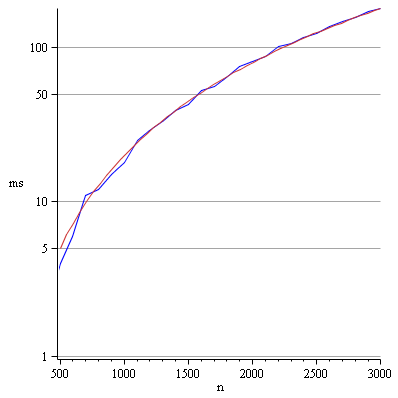
\includegraphics[width=80mm]{RNN_runtime.png}
\caption{The running time of the Reverse Nearest Neighbor algotithm fitted to $x^2$.}
\label{rnn} 
\end{figure}

The blue graph in Figure~\ref{rnn} represents the runtime of our RNN implementation. The orange curve is a fitted $x^2$ function. As expected, the complexity of the algorithm is $O(n^{2})$.

\subsubsection{Global Greedy}

\begin{figure}[ht!]
\centering 
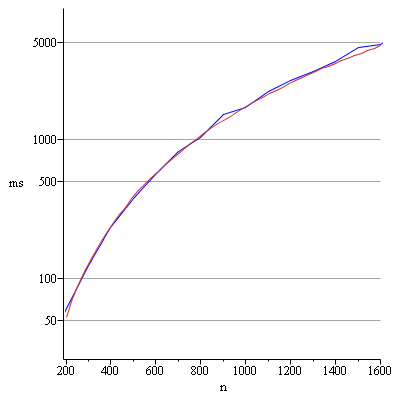
\includegraphics[width=80mm]{GG_runtime.png}
\caption{The running time of the Global Greedy algotithm fitted to $x^2 \cdot log(x)$.}
\label{gg} 
\end{figure}

The blue graph in Figure~\ref{gg} represents the runtime of our GG implementation. The orange curve is a fitted $x^2 \cdot log(x)$ function. As expected, the complexity of the algorithm is $O(n^{2} \cdot log(n))$.

\subsubsection{Stable Marriage}

\begin{figure}[ht!]
\centering 
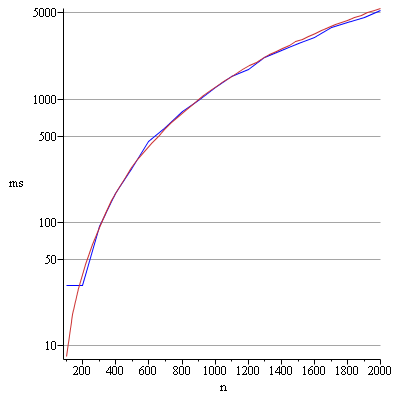
\includegraphics[width=80mm]{SM_runtime.png}
\caption{The running time of the Stable Marriage algotithm fitted to $x^2 \cdot log(x)$.}
\label{sm} 
\end{figure}

\subsubsection{Hungarian Algorithm}

\begin{figure}[ht!]
\centering 
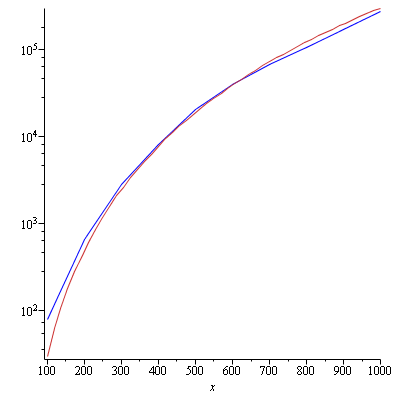
\includegraphics[width=80mm]{HA_runtime.png}
\caption{The running time of the Hungarian algotithm fitted to $x^4$.}
\label{hung} 
\end{figure}

The blue graph in Figure~\ref{hung} represents the runtime of our HA implementation. The orange curve is a fitted $x^4$ function. As expected, the complexity of the algorithm is $O(n^{4})$.

The results of the runtime experiment are provided in Table~\ref{runtimes}. It is clearly seen that because of its simplicity and the early exclusion of nonunique best matches, the Reverse Nearest Neighbour algorithm is the fastest one. The Global Greedy and the Stable Marriage algorithms are noticeably slower. One of the reasons is that the job they are performing differs a bit from the task the RNN is doing. GG and SM are making as many matches as possible, even when there are nonunique smallest distances. They both simply pick one of the possible matches. These two algorithms are also comparable because of the stability of their solutions.

\begin{table}[tbh]
\centering
\begin{tabular}{|c|c|c|c|c|}
\hline 
Size & RNN & Global Greedy & Stable Marriage & Hungarian \tabularnewline
\hline 
\hline 
 100 & 1 & 63 &  & 269\tabularnewline
\hline
 200 & 2 & 159 &  & 640\tabularnewline
\hline 
 300 & 0 & 90 &  & 1826\tabularnewline
\hline 
 400 & 0 & 368 & & 5243\tabularnewline
\hline 
 500 & 2 & 235 &  & 11415\tabularnewline
\hline 
 600 & 4 & 276 &  & 26197\tabularnewline
\hline 
 700 & 5 & 440 &  & 43786\tabularnewline
\hline
 800 & 8 & 961 &  & 85837\tabularnewline
\hline 
 900 & 11 & 1269 &  & 135179\tabularnewline
\hline
 1000 & 17 & 1673 &  & 217143\tabularnewline
\hline 
\end{tabular}
\caption{Running times for different sizes.}
\label{runtimes}
\end{table}

\subsection{Quality Tests}

The recall and precision values of all four algorithms for different datasets are provided in Table~\ref{recall} and Table~\ref{precision}. The interesting remark is that the recall values of GG, SM and Hungarian are very similar in all the cases, and especially of GG and SM. % Discuss the reasons

The other noticeable thing is that for all the algorithms except RNN, the recall and precision values are always the same. Here the explanation is the nature of the algorithms: they always make $min(\#rows, \#columns)$ matches. Therefore the number of false positives becomes equal to the number of false negatives in the formulas of precision and recall. And thus, from the definitions of the precision and recall follows, that precision becomes equal to recall.


\[P = \frac{tp}{tp+fp}, R = \frac{tp}{tp+fn}.\]

\[fp=fn \Rightarrow R=P.\]

\begin{table}[tbh]
\centering
\begin{tabular}{|c|c|c|c|c|}
\hline 
Data File & RNN & Global Greedy & Stable Marriage & Hungarian \tabularnewline
\hline 
\hline 
 Np3q2.dm & 79.26\% & 85.95\% &  & 86.29\%\tabularnewline
\hline
 Nw3p2q.dm & 80.27\% & 89.3\% &  & 89.97\%\tabularnewline
\hline 
 Nw5p1q.dm & 81.94\% & 92.64\% &  & 92.98\%\tabularnewline
\hline 
 Nw8p2q.dm & 82.94\% & 89.97\% &  & 89.63\%\tabularnewline
\hline
\end{tabular}
\caption{Recall of different algorithms for different data.}
\label{recall}
\end{table}

\begin{table}[tbh]
\centering
\begin{tabular}{|c|c|c|c|c|}
\hline 
Data File & RNN & Global Greedy & Stable Marriage & Hungarian \tabularnewline
\hline 
\hline 
 Np3q2.dm & 99.16\% & 85.95\% &  & 86.29\%\tabularnewline
\hline
 Nw3p2q.dm & 98.77\% & 89.3\% &  & 89.97\%\tabularnewline
\hline 
 Nw5p1q.dm & 98.79\% & 92.64\% &  & 92.98\%\tabularnewline
\hline 
 Nw8p2q.dm & 98.41\% & 89.97\% &  & 89.63\%\tabularnewline
\hline
\end{tabular}
\caption{Precision of different algorithms for different data.}
\label{precision}
\end{table}

\section{Conclusions}

\section{Manual}

%-----------------------------------------------------------
\addcontentsline{toc}{chapter}{\numberline{}Bibliography}

\begin{thebibliography}{9999}
%\enlargethispage{\baselineskip}
\bibitem{augsten}
Augsten, N.: Approximate Matching of Hierarchical Data. 
Ph.D. Dissertation, Department of Computer Science Faculty of Engineering and Science Aalborg University
\bibitem{gale}
Gale D.; Shapley L. S., College Admissions and the Stability of Marriage, The American Mathematical Monthly,  69(1): 9–15, 1962.

\bibitem{rnn}
Nikolaus Augsten and Michael B?hlen and Johann Gamper: The pq-Gram Distance between Ordered Labeled Trees, Free University of Bozen-Bolzano, 2010 

\bibitem{ha_firstpub}
Munkres, James: Algorithms for the Assignment and Transportation Problems, Journal of the Society for Industrial and Applied Mathematics, 5(1): pp. 32-38, Mar., 1957

\end{thebibliography}
\vfill
\begin{flushright}\small Prepared in \LaTeXe\ \end{flushright}

%-----------------------------------------------------------
\appendix
\section{Section Name}
%-----------------------------------------------------------
\end{document}
